\documentclass[spanish]{article}
\usepackage[T1]{fontenc}
\usepackage[utf8]{inputenc}
\usepackage{lmodern}
\usepackage[a4paper]{geometry}
\usepackage{babel,amsmath,enumitem,multicol}
\usepackage[]{natbib}
\usepackage{siunitx,tikz,pgfplots,array}
%\usepackage[table]{xcolor}
\usepackage{chemformula}
\usepackage{nicematrix}

\usepackage{pgfgantt}
\definecolor{rojo}{HTML}{ec212d}
\definecolor{azul}{HTML}{273a55}

\begin{document}

	\begin{abstract}
		Investigaremos un problema de transición en el comportamiento de estelas en el flujo alrededor de placas rectangulares. Consideraremos el rol de la relación de aspecto de la placa en la modificación del arrastre asociado para distintos ángulos de inclinación. 
		En el planteo clásico bidimensional del estudio de las fuerzas de arrastre resultantes sobre una placa plana, podemos afirmar que a medida que el ángulo entre la placa y el flujo aumenta --considerando que a $\SI{0}{\degree}$ la placa es paralela  y a $\SI{90}{\degree}$ es normal al flujo incidente-- la fuerza crece en forma monótona. En ese caso, se supone que la dimensión de la envergadura es mucho mayor a la transversal al flujo.  Cuando se introduce una relación finita entre ellas, se tienen las condiciones para que se desarrolle un flujo claramente tridimensional. En este contexto, para altos números de Reynolds ($10^4$) se han medido incrementos de arrastre para ángulos menores a \SI{90}{\degree}. Nuestro objetivo será confirmar experimentalmente dichas medidas y proponer un modelo para la caracterización del escenario de transición.
		 en la estela.
	\end{abstract}
	
	\subsection*{Estado actual del conocimiento}
	
	El flujo alrededor de una placa plana es un flujo prototipo para el estudio de flujos con desprendimiento de la capa límite. A través de este problema, se encuentran importantes aplicaciones en ingeniería y en ciencias ambientales. La configuración puede asimilarse a flujos aerodinámicos si el ángulo  de ataque considerado es bajo, típicamente menor a $\SI{10}{\degree}$.	En tal caso, no hay fenómeno de desprendimiento y dominan las fuerzas de fricción. A medida que consideramos mayores ángulos, el flujo es semejante al que ocurre alrededor de cuerpos romos, la capa límite se desprende y dominan las fuerzas de presión. A menos que lo aclaremos, en lo sucesivo consideraremos al flujo para los casos en que sucede desprendimiento. Si definimos $\ell$ como la longitud de la dirección transversal al flujo, en este caso definimos al número de Reynolds según $\mathrm{Re}=U\ell/\nu$ para una velocidad $U$ y viscosidad cinemática del fluido en cuestión.
	
	\citet{kirchhoff1869theorie} realizó las primeras estimaciones teóricas de la fuerza resultante sobre una placa plana normal al flujo. Más tarde, \citet{rayleigh1911xxiii} completó los cálculos incluyendo predicciones sobre la placa inclinada. Estos resultados no encontraron confirmación en las medidas experimentales hasta que \citet{fage1927flow} extendieron la teoría de \citet{vonkarman1911} sobre las fuerzas en estelas a través de expresiones resultantes de la teoría de flujo potencial. Se consiguió un arreglo a la teoría a partir de la medida de la velocidad en las capas de vórtices de placas inclinadas puede ser mayor a la velocidad de flujo libre, luego la presión resulta menor detrás del cuerpo a diferencia del valor adoptado en la teoría clásica. Consiguieron explicar los valores más altos de arrastre que se obtienen en los experimentos.
		Paralelamente, se publicaron  en Alemania los resultados experimentales de \citet{flachsbart1932} que avanzó sobre la influencia de la relación de aspecto en la performance de sustentación y de arrastre de las placas planas.
	
	
	Más adelante, \citet{kiya1977contribution} elaboraron un modelo invíscido para caracterizar el desprendimiento y la calle de vórtices formada detrás de la placa. En \cite{najjar1995effects, najjar1998low} se interesaron por el carácter tridimensional para el flujo normal a una placa infinita. También \cite{saha2007far} encontraron relaciones para la transición en la estela lejana en el flujo normal a la placa, en forma similar a la hallada en otras geometrías de cuerpo romo. En un trabajo de simulación directa, \cite{yang2012vortex}, caracterizaron inestabilidades de estela de placas inclinadas debidas a la asimetría entre los bordes de ataque, postulando que tal resultado se mantendría aún a mayores números de Reynolds que los ensayados ($\mathrm{Re}\sim100$). Algunos de estos aspectos fueron estudiados en un contexto más general de flujos de estelas por \cite{panesar2023oblique}.

	\cite{gomez2022wake} estudiaron la estela de la placa finita normal e inclinada con respecto al flujo incidente con condiciones de borde de pared y libre, para distintas relaciones de aspecto. Caracterizaron el flujo en forma experimental, determinando intensidad y posición de vórtices. \cite{satheesh2019effect} estudiaron la influencia de la distancia de una superficie libre, para el ensayo de una placa normal al flujo en un canal de agua para distintas relaciones de aspecto.
	
	En un reciento trabajo, \citet{shademan2020effects} estudiaron el efecto de la relación de aspecto sobre el arrastre a través de simulaciones Large Eddy Simulation. Los autores afirman que para una relación 0,5 y un ángulo de \SI{30}{\degree} el arrastre y la sustentación muestran  un comportamiento \textit{irregular} para esa específica combinación de parámetros. Existe un antecedente, ignorado por los autores y, aparentemente, por la mayoría de los trabajos en el tema, que trabajó específicamente sobre las fuerzas de arrastre, la inclinación de la placa y la relación de aspecto. La única publicación, a nuestro saber, que la menciona es la obra de \citet{flachsbart1932}, en alemán, que señala el  estudio experimental que Gustave \citet{eiffel1907recherches} llevó adelante en el Campo de Marte,   \textit{``Recherches exp{\'e}rimentales sur la r{\'e}sistance de l'air ex{\'e}cut{\'e}es {\`a} la tour Eiffel''}.	
	
	Más allá del interés histórico de rescatar los datos experimentales de Eiffel, sus mediciones de fuerza revelan una interesante relación entre la inestabilidad de estela bidimensional y tridimensional. Los resultados, que pueden apreciarse en la Figura \ref{fig:eiffel} nos muestran un escenario de transición para la medida de presión en función del ángulo de inclinación para distintas relaciones de aspecto. Dicha medida, tomada en la estela de la placa, está en estrecha relación con la fuerza de arrastre. En efecto, mientras que para una placa de \textit{infinita } relación de aspecto, la curva I muestra una evolución monótona de incremento del arrastre con el ángulo, la curva IV, por el contrario, exhibe un máximo para valores cerca de los \SI{30}{\degree}. Además de ello, las curvas II y III también tienen asociado, aunque más atenuado, el mismo comportamiento. Es nuestro interés confirmar experimental y numéricamente dichas medidas y tratar de elaborar un modelo para la inestabilidad.
	
	\begin{figure}\centering
	\begin{tikzpicture}
		\node[] (fig) {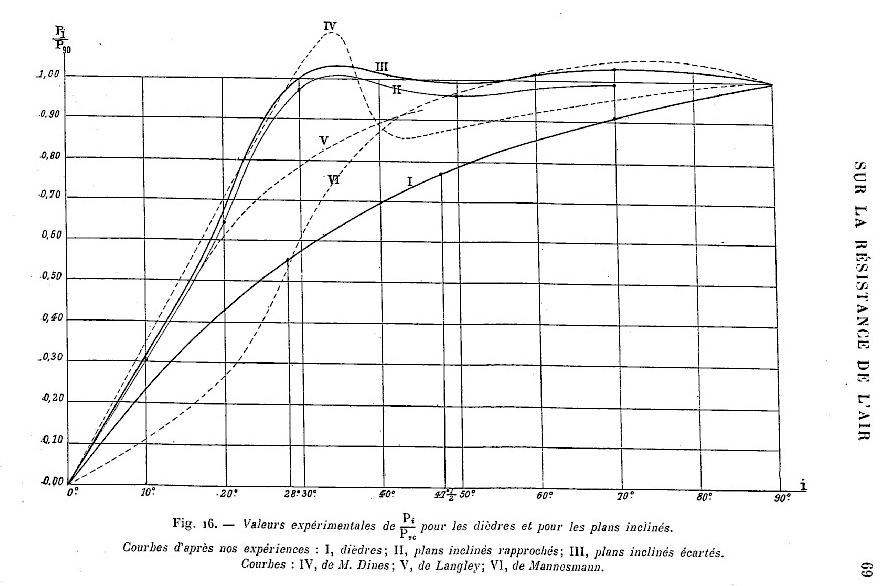
\includegraphics[width=.6\textwidth]{tikzs/eiffel1907}};
	\end{tikzpicture}
		\caption{Medidas experimentales de G. Eiffel (1907).}\label{fig:eiffel}
	\end{figure}

	
	

	
	\subsection*{Objetivos}
	A través del presente trabajo se busca caracterizar la relación entre las fuerzas que se desarrollan para el flujo alrededor de placas planas respecto de distintos ángulos de incidencia y relaciones de aspecto. Por un lado trataremos de confirmar las medidas experimentales de \citeauthor{eiffel1907recherches} y las más recientes simulaciones de \citeauthor{shademan2020effects}.
	Analizaremos trabajos teóricos\citep{fage1927flow,abernathy1962flow,kiya1977contribution} sobre el cálculo de fuerzas, su relación con el arreglo e intensidad de vórtices a través de  modelos no viscosos.  Trataremos  de extenderlos y proponer una ley para caracterizar la inestabilidad que se da para \SI{30}{\degree}.
	
	
	\subsection*{Metodología}
	
	Se propone un abordaje principalmente experimental en el marco de la beca, si bien dentro de los alcances generales del trabajo se propondrá un modelo físico del problema.
	Para ello se cuenta con instalaciones del Canal de Experiencias de Arquitectura Naval de la Facultad de Ingeniería de la Universidad de Buenos Aires. Se trata de un canal hidrodinámico de superficie libre de 72 m de largo que esencialmente se destina a experiencias de modelos reducidos de barcos y de sistemas de propulsión. Posee
	un generador de ondas que permite propagar olas de diferentes amplitudes y longitudes de onda. Cuenta con un carro de ensayos que soportará el modelo y lo desplazará a lo largo del canal. Pueden realizarse medidas de fuerzas de arrastre, sustentación así como también el  torque sobre la placa.
	
	Un medida complementaria la haremos mediante el uso de cámaras rápidas, a fin de determinar la frecuencia principal de desprendimiento de vórtices en la estela.
	
	Las maquetas de las placas de distinta relación de aspecto  se realizarán en polimetil metacrilato (PMMA). Diseñaremos el soporte que vincule la placa al carro y la posibilidad de fijar los distintos ángulos de ataque.
	
	Por último, haremos simulaciones numéricas directas del fenómeno a partir del software libre Basilisk\cite{popinet2014basilisk}.  Estudiaremos la posibilidad de extender cálculos a moderados números de Reynolds pero que resuelvan el problema en tres dimensiones.
	\subsection*{Antecedentes en el tema}
Durante los últimos años hemos trabajado sobre temas de investigación de 
control e inestabilidades en mecánica de fluidos. En particular, nos hemos interesado en  
de flujos de estela. En 
general nuestros estudios se basaron en el control activo, es decir a partir de 
la introducción de un actuador (plasma, mecánico, de inyección de fluido) capaz 
de modificar el flujo.  Distintos fenómenos que aparecen en el flujo 
alrededor de un ala flexible, han sido tratados en nuestros trabajos. El 
control de flujos con separación \cite{dadamo2014a}, 
estabilización de las fluctuaciones en estela 
\cite{dadamo2017a,castro2020vortex}, el estudio de la modificación de la 
fuerzas resultantes sobre el cuerpo \cite{sosa2009a,dadamo2011b,sosa2013}, la optimización de la interacción fluido sólido en propulsión de placas flexibles\cite{dadamo2022wake}, la 
construcción de modelos reducidos para el control e inestabilidad de estelas
\cite{boury2018forced}.

Por último, cabe mencionar que nuestro laboratorio forma parte del Laboratorio 
Internacional Asociado (IRL),  Instituto Franco-Argentino de Dinámica de FLuidos para el Medio Ambiente (IFADyFE) creado por el CNRS de Francia, la UBA y Conicet. El presente trabajo se enmarca entre los ejes principales de colaboración, en relación al ahorro energético que puede conseguirse en este tipo de escurrimientos. Se supone un paso inicial a la posibilidad del control a través de interacción fluido estructura. 
	\subsection*{Cronograma}
 	\begin{ganttchart}[
 	y unit title=0.5cm,
 	y unit chart=0.5cm,
 	x unit =0.75cm,
 	vgrid,hgrid,
 	title height=1,
 	title/.style={fill=none},
 	title label font=\footnotesize,
 	bar/.style={fill=gray!60},
 	bar height=1,
 	bar top shift=0,
 	progress label text={},
 	group right shift=0,
 	group height=.1,
 	group peaks width={0.2},
 	inline, 
 	bar label node/.style={text width=3.5cm,
 		align=right,
 		anchor=east,
 		font=\small}
 	]{1}{12}
 	
 	\gantttitle{\textcolor{rojo}{2024}}{3}|
 	\gantttitle{\textcolor{azul}{2025}}{9} \ganttnewline 
 	\gantttitle{Oct}{1} \gantttitle{Nov}{1} \gantttitle{Dic}{1} \gantttitle{Ene}{1} 
 	\gantttitle{Feb}{1} \gantttitle{Mar}{1} \gantttitle{Abr}{1}
 	\gantttitle{May}{1} \gantttitle{Jun}{1} \gantttitle{Jul}{1}\gantttitle{Ago}{1}\gantttitle{Sep}{1}\\
 	
 	\ganttbar[progress=100,inline=false]{1.}{1}{4} {5}{12}	\\
	\ganttbar[progress=100,inline=false]{2.}{1}{2} 	\\
	\ganttbar[progress=100,inline=false]{3.}{2}{2} 	\\
	\ganttbar[progress=100,inline=false]{4.}{3}{4} 	\\
	\ganttbar[progress=100,inline=false]{5.}{4}{4} 	\\
	\ganttbar[progress=100,inline=false]{6.}{5}{6} 	\\	 
	\ganttbar[progress=100,inline=false]{7.}{6}{7} 	\\	 
	\ganttbar[progress=100,inline=false]{8.}{6}{8} 	\\	 
	\ganttbar[progress=100,inline=false]{9.}{7}{11}	\\	 	
	\ganttbar[progress=100,inline=false]{10.}{10}{12}	
 \end{ganttchart}
 

	
\begin{multicols}{2}
	\begin{enumerate}[nosep]
	\item Estudio bibliográfico.		
	\item Diseño y realización de la maqueta del soporte de placas en el carro de mediciones del Canal.
	\item Diseño y uso de  trazadores pasivos en la estela.
	\item Toma de medidas de fuerza.
	\item Toma de video con cámara rápida.
	\item Análisis y presentación de primeros resultados de fuerzas.
	\item Post-procesamiento de imágenes y análisis de medidas de frecuencias principales del flujo.
	\item Análisis de resultados, planteo  de simulaciones numéricas 
	complementarias en Basilisk.
	\item Elaboración de un modelo físico y contraste con las medidas experimentales y numéricas.
	\item Preparación de publicación.
\end{enumerate}

\end{multicols}	
	\bibliography{/home/juan/Documents/bibtex/citas}
	\bibliographystyle{apalike}  
	
\end{document}


 
